\pdfminorversion=5 % To enforce 1.5 version of PDF
% Preamble
% =============================================================
\documentclass[xcolor=table]{beamer}        % Just Slides
%\documentclass[xcolor=table,notes]{beamer} % Slides and Notes


% Encoding
% =============================================================
\usepackage[english]{babel}
\usepackage[latin1]{inputenc}


% Beamer Class Template Settings
% =============================================================
\usetheme[compress]{Dresden}
\setbeamercovered{transparent}
\usefonttheme[onlysmall]{structurebold}
\beamertemplatenavigationsymbolsempty
\useinnertheme[shadow=true]{rounded}
\usefonttheme[onlymath]{serif}


% Packages
% =============================================================
\usepackage{color}
\usepackage{colortbl}
\usepackage{ziffer}
\usepackage{amsmath,amsfonts,amssymb}
\usepackage{etex}
\usepackage[absolute,overlay]{textpos}
\usepackage{framed}
\usepackage{media9}
\usepackage{hyperref}

\hypersetup{
pdfstartview={Fit},
bookmarks=True,
pdftitle={Git Workshop},
pdfauthor={Nicolas Guarin-Zapata, Cyrus Vandrevala},
pdfsubject={Lectures},
pdfkeywords={Version control, Scientific Computing}
}


% Definitions
% =============================================================
\setlength{\TPVertModule}{\paperheight}
\setlength{\TPHorizModule}{\paperwidth}
\setlength{\TPHorizModule}{\paperwidth}\setlength{\TPVertModule}{\paperheight}

\setbeamercolor{footlinecolor}{bg=RUBgrau,fg=RUBblau}

% Footline Information
\setbeamertemplate{footline}{
  \begin{beamercolorbox}[sep=1em, wd=\paperwidth,leftskip=0.4cm,rightskip=0.4cm]{footlinecolor}
  \mbox{
    \begin{minipage}{0.2\paperwidth}
	  
\includegraphics[width=0.1\paperwidth]{img/Purdue-logo-BW2.pdf}
	\end{minipage}
	\begin{minipage}{0.6\paperwidth}
	  \begin{center}
	    Git Workshop
	  \end{center}
	\end{minipage}
	\begin{minipage}{0.2\paperwidth}
	  \scriptsize{\insertframenumber}
	\end{minipage}}
  \end{beamercolorbox}
}


% Colors
% =============================================================
\definecolor{RUBgrau}   {HTML}{e6e4e4}
\definecolor{RUBblau}   {HTML}{003560}
\definecolor{RUBgruen}  {HTML}{94c11c}
\definecolor{middlegray}{rgb} {0.5,0.5,0.5}
\definecolor{lightgray} {rgb} {0.97,0.97,0.97}
\definecolor{tablegray} {rgb} {0.85,0.85,0.85}
\definecolor{white}     {rgb} {1.0,1.0,1.0}
\definecolor{orange}    {rgb} {0.8,0.3,0.3}
\definecolor{yac}       {rgb} {0.6,0.6,0.1}
\definecolor{red}       {rgb} {1.0,0,0}
\definecolor{green}     {rgb} {0.0,1.0,0.0}
\definecolor{black}     {rgb} {0,0,0}
\definecolor{blue}      {rgb} {0,0,1.0}
\definecolor{lightblue} {rgb} {0.5,0.9,1.0}


% Beamer Class Color Settings
% =============================================================
\setbeamercolor{block body example}{bg=RUBgrau}
\setbeamercolor{block title example}{bg=RUBblau,fg=white}
\setbeamercolor{block body alerted}{bg=RUBgrau}
\setbeamercolor{block title alerted}{bg=red,fg=black}

\setbeamercolor{section in head/foot}{fg=white, bg=RUBblau}
\setbeamercolor{subsection in head/foot}{fg=black, bg=white}
\setbeamercolor{block title}{fg=RUBblau}
\setbeamercolor{section in toc}{fg=RUBblau}
\setbeamercolor{section}{fg=RUBblau}
\setbeamercolor{item}{fg=RUBblau}
\setbeamercolor{frametitle}{fg=RUBblau,bg=RUBgrau}
\setbeamercolor{framesubetitle}{fg=black}
\setbeamercolor{title}{fg=RUBblau,bg=RUBgrau}
\setbeamercolor{titlelike}{bg=RUBblau}

\setbeamercolor{palette sidebar primary}{use=normal text,fg=normal text.fg}
\setbeamercolor{palette sidebar quaternary}{use=structure,fg=structure.fg}
\setbeamercolor{palette sidebar secondary}{use=structure,fg=structure.fg}
\setbeamercolor{palette sidebar tertiary}{use=normal text,fg=normal text.fg}

\setbeamercolor{section in sidebar}{fg=RUBgrau}
\setbeamercolor{section in sidebar shaded}{fg=RUBgrau}
\setbeamercolor{separation line}{}
\setbeamercolor{sidebar}{bg=RUBgrau}
\setbeamercolor{sidebar}{parent=palette primary}


% Title Page Customization
% =============================================================
\setbeamertemplate{title page}{
  \vspace{0.25cm}
  \begin{columns}
    \column{.6\textwidth}
      \insertsubtitle\\
	  \vspace{0.5cm}
	  {\usebeamerfont{title}\usebeamercolor[fg]{title}\inserttitle}\\
	  \vspace{0.5cm}
	  \insertauthor\\
	  \vspace{2mm}
	  \insertdate
	  \vfill
    \column{.4\textwidth}
	\begin{center}
	  
\includegraphics[width=0.9\textwidth]{img/Git-logo}\\
	  \vspace{3mm}
	  
\includegraphics[width=0.9\textwidth]{img/github_logos/GitHub_Logo}\\
	  \vspace{3mm}
	  
\includegraphics[width=0.9\textwidth]{img/Purdue-logo-BW2}
    \end{center}
  \end{columns}
}



% TITLE PAGE PARAMETERS
\title{Workshop: Git and GitHub (Day 2)}
\subtitle{~}
\institute{Purdue University}
\author[AUTHOR]{\scriptsize{Cyrus Vandrevala $^1$\\Nicol\'as Guar\'in-Zapata$^2$}\\
\tiny{$^1$ Physics Department\\ $^2$ Civil Engineering Department}}
\date{\today}


% ===================================================================== %
% CHAPTER 0 : Title page and overview
% ===================================================================== %
\begin{document}

% INTRODUCTION
% ======================================= %
% TITLE SLIDES
% ======================================= %

\begin{frame}[plain]
\titlepage
\end{frame}
\note{}

\begin{frame}
\frametitle{\large{Overview}}
\tableofcontents
\end{frame}
\note{}

\begin{frame}
\frametitle{\large{We Encourage Participation!}}
\begin{itemize}
\item Post Questions That You Might Have in the Repo
\item Recommend Other Sources That You Found Useful
\item Remember, We Do Not Know Everything!
\end{itemize}
\end{frame}
\note{}


% ======================================= %
% GITHUB PAGES
% ======================================= %
\section[GitHub Pages]{GitHub Pages and Jekyll}

\begin{frame}
    \frametitle{Pages}
    
    \begin{enumerate}
    \item GitHub allow users to have one personal (static) site. \pause
    
    \item Allows a site per project. \pause
    
    \item Jekyll is the site-generator behind GitHub Pages. There are plenty of templates written in Liquid. \footnote{See here \url{http://jekyllrb.com/docs/templates/}. If you are one of those geeks... you can also use CSS templates.}

    \end{enumerate}
\end{frame}
\note{}      

% ======================================= %
% GITHUB MOBILE APP
% ======================================= %
\section[Mobile App]{GitHub Mobile App}

\begin{frame}
    \frametitle{Mobile App}
\begin{columns}[c]
\column{2in}
	\centering
	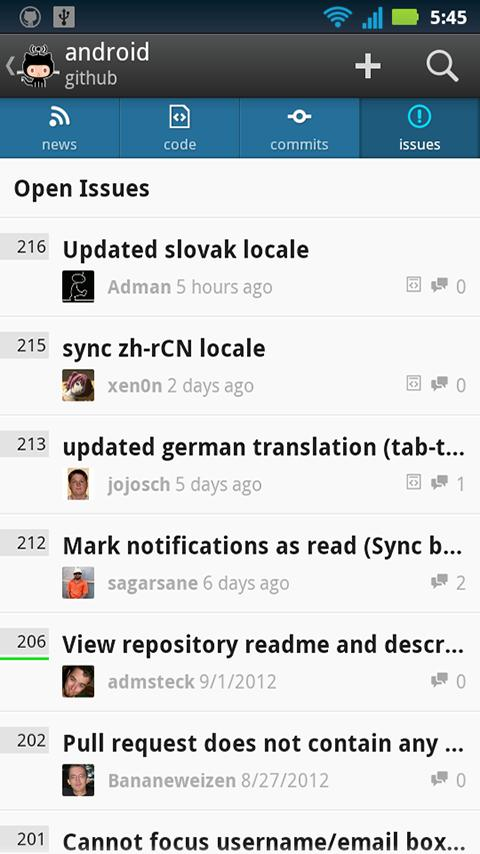
\includegraphics[width=1in]{img/mobile.jpg} 
\column{2in}
GitHub for Android\footnote{https://mobile.github.com/}
\begin{enumerate}
\item Issue Dashboard.
\item Gist Support.
\item News Feed.
\end{enumerate}
\end{columns}
\vspace{5mm}
{\small Off course, it is not a replacement for a Desktop client. But it is good enough to keep track of some changes on the go.}
\end{frame}
\note{}

% ======================================= %
% GITHUB EDUCATION
% ======================================= %
\section[GitHub Education]{GitHub Student Developer Pack (GitHub Education)}

\begin{frame}
    \frametitle{GitHub Student Developer Pack}
      
    A couple of months ago GitHub (with some companies) released a pack of free tools for students\footnote{https://education.github.com/pack}. Here we present some of them that were arbitrarily chosen.
    
    \begin{enumerate}    
    \item Atom: a text editor developed by GitHub. \pause
    
    \item CrowdFlower: data enrichment, data mining and crowdsourcing services. \pause
    
    \item GitHub: 5 Private GitHub Repos. \pause
    
    \item SendGrid: Email services. \pause
    
    \item Unreal Engine: A suite of game development tools for PC, console, mobile and web.
    \end{enumerate}

\end{frame}
\note{}    

% ======================================= %
% GITHUB OPENSOURCE PROJECTS
% ======================================= %
\section[Open Source]{GitHub Open Source Projects}
\begin{frame}
    \frametitle{GitHub Open Source Projects}
    
\begin{itemize}    
	\item Jekyll: https://github.com/jekyll/jekyll \pause
        
    \item Linux Kernel: https://github.com/torvalds/linux \pause
    
    \item Matplotlib: https://github.com/matplotlib/matplotlib\pause
        
    \item Scipy Lecture Notes: https://github.com/scipy-lectures/scipy-lecture-notes
    
\end{itemize}   

\end{frame}
\note{}

\begin{frame}
    \frametitle{Cool stuff}
    
    \begin{itemize}
    \item D3: \url{https://github.com/mbostock/d3} \pause
    
    \item Flatland (Book): \url{https://github.com/Ivesvdf/flatland} \pause
    
    \item Generate DOI for Github Repos: \url{https://guides.github.com/activities/citable-code/} \pause 

    \item GitBook (Books Editor): \url{https://www.gitbook.io/} \pause
     
    \item GitHub Visualizer: \url{http://ghv.artzub.com/} \pause
       
    \item ShareLatex: \url{https://github.com/sharelatex/sharelatex}
    \end{itemize}
\end{frame}
\note{}

% ======================================= %
% GITHUB COMMUNITY
% ======================================= %
\section[GitHub Community]{GitHub Community}
\begin{frame}
    \frametitle{GitHub Community}
    
    \begin{itemize}
    \item Choosing an OSS license: \url{http://choosealicense.com/} \pause
    
    \item GitHub Explore: https://github.com/trending \pause
    
    \item Gitter: Chat rooms for GitHub Projects (\url{https://gitter.im})
    
    \item LearnProgramming: \url{http://learnprogramming.github.io/}   
    
    \end{itemize}
\end{frame}
\note{}

% ======================================= %
% PROGRAMMING EXAMPLE
% ======================================= %
\section[Example]{Programming Example}
\begin{frame}[allowframebreaks]
    \frametitle{Verlet Integration}
    
Verlet integration is a numerical method used to integrate Newton's equations of motion. It is frequently used to calculate trajectories of particles in molecular dynamics simulations and computer graphics.

If we do a Taylor expansion of the position vector $\vec{x}(t\pm\Delta t)$ forwards and backward we get
\begin{align*}
\vec{x}(t + \Delta t)
&= \vec{x}(t) + \vec{v}(t)\Delta t + \frac{\vec{a}(t) \Delta t^2}{2}
+ \frac{\vec{b}(t) \Delta t^3}{6} + \mathcal{O}(\Delta t^4)\\
\vec{x}(t - \Delta t)
&= \vec{x}(t) - \vec{v}(t)\Delta t + \frac{\vec{a}(t) \Delta t^2}{2}
- \frac{\vec{b}(t) \Delta t^3}{6} + \mathcal{O}(\Delta t^4), \,
\end{align*}
Adding these two expansions gives
\[\vec{x}(t + \Delta t) = 2\vec{x}(t) - \vec{x}(t - \Delta t) + \vec{a}(t) \Delta t^2 + \mathcal{O}(\Delta t^4)\, .\]
We can see that the first and third-order terms from the Taylor expansion cancel out, thus making the Verlet integrator an order more accurate than integration by simple Taylor expansion alone.

So we can use as time stepper the equation
\[\boxed{\vec{x}(t + \Delta t) = 2\vec{x}(t) - \vec{x}(t - \Delta t) + \vec{a}(t) \Delta t^2} \enspace ,\]
or in terms of forces
\[\boxed{\vec{x}(t + \Delta t) = 2\vec{x}(t) - \vec{x}(t - \Delta t) + \frac{\vec{F}(t)}{m} \Delta t^2} \enspace ,\]

Our goal is to create a solver for Newton equations using Verlet integration. We can split the project into small groups. A possible division of labors is
\begin{itemize}
\item Force routines (springs, electrostatic interactions, some wacky stuff);

\item Verlet step calculator for different coordinates $x$, $y$ and $z$;

\item Verlet time stepper;

\item Plotting capabilities; and

\item Main routines.
\end{itemize}
    
\end{frame}
\note{}

% ======================================= %
% PROGRAMMING CHALLENGES
% ======================================= %
\section[Challenges]{Programming Challenges}
\begin{frame}
    \frametitle{Small programming tasks}    
    
We have a set of \emph{simple} programming tasks. The main idea is to get a set of different solutions to compare the execution times or the codes. Please commit your code as \texttt{probX\_ID.ext}, where \texttt{X} is the number of the problem, \texttt{ID} and \texttt{ext} is the extension of the file. There is a directory named \texttt{./programming\_challenges/}, where you should commit your solutions.

\end{frame}


%% Ending
\begin{frame}
    \frametitle{\large{}}
    \huge{\center{\color{RUBblau}{Thank you for your attention.}}}
\end{frame}

\end{document}
\note{}